\documentclass[10pt,conference]{IEEEtran}
\usepackage{lipsum} % for filler text
\usepackage{graphicx,float} % graphics please
%
% Need to make graphics? Use Inkscape: https://inkscape.org/
% Need something simpler and collaborative? https://www.draw.io/
%
\usepackage{fancyhdr}
\usepackage[acronym]{glossaries}
\makeglossaries
\usepackage{amsmath,amssymb}
\pagestyle{fancy}
\fancyhead{} % clear all header fields
\renewcommand{\headrulewidth}{0pt} % no line in header area
\fancyfoot{} % clear all footer fields
\fancyfoot[LE,RO]{\thepage}           % page number in "outer" position of footer line
\fancyfoot[RE,LO]{\it Not for Public Distribution.} 
\usepackage[utf8]{inputenc}

\usepackage{xcolor} % used for highlighting things for me to come back to

\title{Evolutionary Intrusion Detection System for Controller Area Networks}
\author{Robert Jared Clark \\
Michigan State University \\
East Lansing, Michigan 48824 \\
Contact: clarkr28 at msu dot edu}
\date{\today}

\begin{document}

\maketitle

\begin{abstract}
The purpose of the work presented in this paper was to determine if Evolutionary Computation (EC) can be used to evolve rules for a CAN-based Intrusion Detection System (IDS).  An Intrusion Detection System is only as good as the rules that govern it, which requires expert knowledge to make by hand.  Consequently, Genetic Programming (GP) was thought of as a possible way to evolve optimal rules, which does not require expert knowledge of the system. Details of our Genetic Programming implementation are given and preliminary results presented based on the ability to detect denial of service and fuzzy attacks on CAN networks.  We conclude by determining that our implementation does not generate IDS rules that perform with a high enough accuracy to recommend their use in governing an IDS.
\end{abstract}

\section{Introduction}

% Introduction Paragraph
Modern vehicles are being built with an increasing amount of technology to support more advanced features for consumers.  This technology is realized in the form of Electronic Control Units (ECU), which typically communicate over Controller Area Networks (CAN).  CAN networks are notoriously insecure, and therefore pose a significant security risk to modern vehicles.  A first line of defense is simply knowing if a network is under attack, which is the role of an Intrusion Detection System (IDS).  An IDS uses rules, or some form of predefined knowledge, to process network traffic with the goal of detecting irregular or malicious behavior.  The performance of an IDS is dependent on its rules, and therefore the formation of these rules are of significant importance.  This paper presents an applied analysis to determine if rules for an IDS can be evolved with Genetic Programming.

% Background Paragraph
Many researchers have focused on ways to create Intrusion Detection Systems, some for CAN networks, but more frequently for TCP/IP networks.  Kang and Kang created an IDS for CAN networks that processed messages using a deep neural network (DNN) to predict if the message was part of an attack\cite{kang2016intrusion}.  The combination of feature extraction and DNNs used in this work was able to achieve an impressive average detection accuracy of 98\%.  The time it took to process a message was also low, reporting 8-9 $\mu$s for feature extraction and 2-5 ms for classification.  However, the hardware used was not included, which could drastically affect computation time.  In a different work, Hoque et al. used evolutionary computation to evolve an IDS for a TCP/IP netowrk\cite{hoque2012implementation}.  While their implementation had a high detection rate of 99\% for denial of service attacks, performance was significantly lower for all other attack types.  As a loose extension of their work, this paper presents a genetic programming implementation for evolving rules to be used in a CAN-based IDS.  

% Transition Paragraph - what keen insight did you apply to overcome others shortcomings
Although a well-trained DNN can classify nonlinear data with high accuracy, processing power is a sharp limitation with all vehicles.  Even though a DNN-based IDS would be trained separately, the time required to propagate a CAN message through a DNN could break the real time requirement of CAN networks.  However, the processing of CAN message features presented in this paper does not involve feature selection or DNN propagation, and therefore should be faster.  The larger question for this work to identify is if this method will be able to detect injected CAN messages at a high enough rate.

% Details Paragraph - Technical challenges and validation methods
There are many design decisions that need to be made for genetic programming to be implemented, the first of which is how to encode a genome.  Significant differences exist between TCP/IP and CAN networks, and as a result, the genome evolved in this work had to be significantly different than the work done by Hoque et al. \cite{hoque2012implementation}.  For instance, CAN networks do not have IP addresses, or any means of identifying where a message is from and what ECU it is for.  CAN networks also have no built in way to track how many messages have been sent by a given source.  Both of these elements are used in a TCP/IP-based IDS, and there is no straightforward parallel that could be implemented on a CAN network.  Therefore, the genome's structure had to be modified in order to work for a CAN network.  However, it became evident that different genomes performed better for different CAN attack types, as will be discussed in future sections.  Another significant design decision that had to be made in order to implement an EA was the goals of the fitness function.  In order to generate rules for a CAN-based IDS, the fitness function was structured to reward genomes that match with attack messages and penalize messages that match with normal messages, which should push the overall population towards evolving ideal solutions.  

% Assessment Paragraph - Assess results, state conclusions, map out remaining sections
When considering the results generated by this implementation, the IDS rules evolved did not yield a high enough accuracy to warrant their use in a real CAN-based IDS.  Future work could be done to improve on this implementation, and this work could be used as a baseline comparison or a starting place to branch.  The remaining sections proceed as follows: section 2 overviews background information and related work, section 3 describes the methodology of our implementation, section 4 discusses the results and performance of the evolved IDS rules, section 5 draws conclusions and proposes future work.

\section{Background and Related Work}

The primary goal of Genetic Programming is to evolve an optimal program or part of a program. The underlying idea lies in the basis of biological evolution where individuals can have unique characteristics stemming from their DNA that give them advantages or disadvantages in comparison to the rest of the population.  Those with more advantages will survive longer and pass their traits to their offspring.  

A critical component of any Evolutionary Algorithm is its genome.  For a Genetic Algorithm (GA), a typical genome could be a sequence of bits, numbers, or characters within a given range that can evolve and mutate.  The components of a GA's genome would be used in some part of a program or agent and would have an affect on the way it behaves.  With GP, the genome is some form of code.  Some forms of GP will have a genome consisting of computer instructions, such as adding two registers, where the instruction is executed directly in a process.  What is more frequently observed with an evolutionary IDS is to have a GP genome that essentially defines the \textit{if} condition for an \textit{if else} structure that defines anomalous network behavior.  

After genomes, fitness functions are the next logical element of an EA to consider.  The fitness function generates a value for every individual based upon how well its genome can performs the required tasks.  This fitness value is then used to rank the individuals, which affects the likelihood that they will advance to the next round.  This process of picking the more fit individuals is what pushes the entire population towards higher fitness values, as the genome of the more fit individuals will possibly mix with other individuals' genomes in subsequent generations.  

Mutation and crossover are the main components that generate new solutions for an EA.  During mutation, values in a genome are randomly changed with a specified probability.  During crossover, sections of two genomes are swapped to create new combinations of offspring genomes.  These changes in genomes will cause a change in the way the genome performs its required tasks.  If the changes are beneficial, the individual now has an advantage over other individuals, and it will likely advance to future generations where it can pass its more optimal genome to its offspring.  

Cyber-security has become a more prevalent concern for modern vehicles as knowledge has increased about the ease at which they can be breached.  Koscher et al. demonstrated the ability to adversely affect vehicles, in which the CAN network was key to their success\cite{koscher2010experimental}.  Their controlled takeover of the vehicle was so successful that they were even able to disable braking and turn off the engine.  

Lu and Traore presented a GP approach to generating IDS rules for an IP network\cite{lu2004detecting}.  Their goal was to detect both known and novel attacks.  Their focus on detecting novel attacks is important, as threats are always evolving.  A notable characteristic of their implementation was that they used a tree-based approach to defining rules, instead of the chromosome-like rules evolved in other papers\cite{hoque2012implementation}\cite{li2004using}.

Pillai et al. proposed another GA for evolving IDS rules for IP networks and chromosome-like rules\cite{pillai2004approach}.  Their work is another instance where the framework was only discussed in theory, and not done in practice to validate.  

\section{Methods}

Genetic Programming implementation details are provided in this section.

\subsection{Data}

For this work, a data source was found that contained various CAN-based attack data sets\cite{candata}.  These data sets were created by logging data from a vehicle's OBD-II port while attack messages were being injected.  Every logged message had a time stamp, arbitration value, message data (0 to 8 bytes), and a flag to classify the message as normal or injected.  The time stamps were not used in this study, but it is noted that these time stamp values could be a valuable addition in future work.  The time stamps were not used as there was not a clear way to incorporate time stamps into fitness values that would encourage the genome to evolve towards more effective solutions.

Two attack types were used in this study - denial of service and fuzzy attacks.  The denial of service attack injects CAN messages of all zeros at a high frequency.  The CAN protocol uses the arbitration value to determine which message to give priority when multiple messages are trying to be sent at the same time.  With an arbitration value of all zeros, the injected messages will always have priority over other messages, preventing genuine messages from being sent.  The fuzzy attack works by injecting messages with random arbitration values and random data.  Both denial of service and fuzzy attack data sets were downloaded and processed by removing time stamps and only keeping unique messages.  Removing duplicate messages drastically reduced the sizes of the data sets.  The denial of service data set originally contained 3.7 million messages and was reduced to 24,273 unique messages.  Similarly, the fuzzy data set originally contained 3.8 million messages and was reduced to 82,773 unique messages.  Notice that there are more unique fuzzy messages than denial of service messages.  This is due to the fact that the injected fuzzy messages contain random (unique) data, while the injected denial of service messages are all zero and therefore the same.  

The fact that all injected denial of service messages are the same makes identifying those messages trivial.  To make the problem slightly harder, the denial of service data set was duplicated.  In the duplicated version of every message, the arbitration value was changed to zero, and the class label was changed to injected.  This way, an optimal genome would have to identify that only the arbitration value is important for denial of service attacks.  

\subsection{Genome}

The genome used for this CAN-based IDS revolves around two parts of the CAN data - the arbitration value and the message data itself.  The genome also had the ability to ignore portions of the arbitration value and message data.  

Two genome versions were made for this experiment.  The first genome was a purely binary genome.  For every bit in the CAN arbitration and message data, the genome would have two bits.  The first bit in the genome would indicate if the piece of CAN data was important for classification, and the second bit in the genome indicated what value to look for in the corresponding CAN data bit.  Figure \ref{binarygenome} gives a graphical representation of how the binary-based genome pairs with CAN data.  The goal of the genome was to match with as many injected CAN messages as possible.  Therefore, the genome would evolve to find patterns of data that only existed in injected messages.  

\begin{figure}[H]
    \centering
    \text{Binary-Based Genome and CAN Data}
    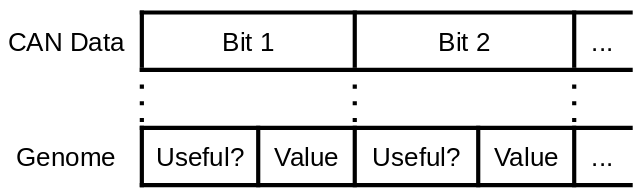
\includegraphics[width=0.5\textwidth]{binary-genome.png}
    \caption{A representation of how the binary-based genome matches with CAN data (bit by bit). Genome elements in both the \texttt{Useful?} and \texttt{Value} sections are binary.}
    \label{binarygenome}
\end{figure}

A second genome was also made that was not purely binary.  Instead of having genome values for every bit in the CAN data, the second genome had values for every section of CAN data, where the arbitration value and every byte of CAN message data was its own section.  As a result, the genome was trying to match with sections of the CAN data instead of bits of the CAN data.  To be clear, the first section of the genome corresponded to the arbitration value, where the genome had a bit to indicate if the arbitration value was important, and if so, what integer value to look for in the arbitration section.  The next section of the genome would correspond to the first byte of CAN message data, where the genome had a bit to indicate if the first byte of CAN message data was important, and if so, what integer value to look for. Figure \ref{integergenome} gives a graphical representation of how the integer-based genome pairs with CAN data.  

\begin{figure}[H]
    \centering
    \text{Integer-Based Genome and CAN Data}
    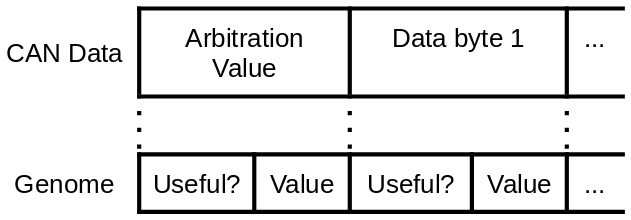
\includegraphics[width=0.5\textwidth]{integer-genome.png}
    \caption{A representation of how the integer-based genome matches with CAN data (section by section). Genome elements in the \texttt{Useful?} section are binary, while elements in the \texttt{Value} section are integers.}
    \label{integergenome}
\end{figure}

\subsection{Message Classification}

The core of any IDS is the way it determines if messages are normal or abnormal.  In this work, as with other previous works \cite{li2004using, hoque2012implementation}, this decision takes the form \texttt{if \{condition\} then \{action\}}, where various parameters of a message are checked in the \texttt{condition} statement and the message is considered abnormal if the \texttt{condition} evaluates to True, triggering some \texttt{action}. 

While this \texttt{if \{condition\} then \{action\}} ideology is the same for both TCP/IP and CAN-based networks, there are significant differences between the two protocols.  As a result, the contents of the \texttt{condition} statements are very different.  Many parameters associated with TCP/IP data do not have parallels with CAN data.  For instance, CAN messages have no destination or origin IP and port addresses, as CAN messages are simply broadcast through the entire network.  TCP/IP connections also track how many packets have been sent and received by both hosts connected.  This kind of tracking does not exist on CAN networks.  All of these TCP/IP values can be used in the \texttt{condition} statement that determines if a packet is irregular and cannot be used in a CAN \texttt{condition} statement because they do not exist.  

It should be noted that this paper is not concerned with the \texttt{action} to perform when a CAN message is detected as malicious, as this is an entirely problem for other research.  The action to perform when a TCP/IP connection is detected as malicious is usually straightforward, namely, the connection is closed.  There is no direct parallel to CAN networks because CAN networks broadcast messages through the entire network.  Therefore, CAN networks do not have connections between ECUs that can simply be closed to prevent them from communicating.  This is a nontrivial problem that deserves investigation.  

Message classification for CAN messages in this implementation works as follows.  For a given evolved genome, all training messages are computed against the genome to generate an integer value for every message indicating how closely the message matches the genome (see Genome subsection for more details about the genome).  The average of these values are then computed for both normal and injected messages.  Remembering that an optimal genome should match highly with the injected messages and match minimally with the normal messages, the distance between the two average values is an indication of how well the genome has distinguished between the two classes.  The middle of the two averages is then used as a decision boundary to classify future messages as either normal or injected.  

\subsection{Fitness Function}

A final area of implementation to be discussed is the fitness function.  The fitness function is very similar to how message classification works.  The fitness function and message classification algorithm both start by taking can messages and computing a value for every message quantifying how well the genome matches with the message.  Next, if the message is from the injected class, the value is added to the overall fitness value.  Otherwise, the message is from the normal class, and the value is subtracted from the overall fitness value.  This setup rewards genomes for matching with injected messages and penalizes genomes for matching with normal messages. 

\section{Results}

Evolutionary runs were performed on fuzzy data and denial of service data separately, and consequently, the results are presented separately.  

\subsection{Fuzzy Attack}

Many evolutionary runs were done with the fuzzy attack data set, and the set of runs that produced the best results are displayed in Table 1.  From the table, the mutation rate displays the percent chance that any bit in the binary genome will be flipped.  The test size represents how many randomly selected messages the genomes were evaluated with to generate fitness values.  Keep best represents how many of the fittest individuals were copied to the next generation without mutation.  This was done as a measure to preserve the best-performing individuals.  The maximum train and test percentages represent the highest accuracy rates from the final generation of evolved individuals.  The maximum fitness values represent the highest fitness value observed through the duration of the run.  

The population size, number of generations, and testing size were kept constant through the evolutionary runs presented in Table 1.  These values were limited to the values displayed in Table 1 because they have a direct affect on run time.  Many of the other runs not mentioned in this paper had a combination of smaller population, generation, and test sizes. The results presented here were one of the final runs performed, and they had the largest combination of the three values.  

An interesting observation from the data presented in Table 1 is that the run that produced the highest fitness value was not the run that had the highest training and testing accuracy.  In fact, the run with the highest training and testing accuracies had the fifth highest maximum fitness value.  The maximum fitness values from Table 1 shows that as the mutation rate increased, the maximum fitness value decreased without exception.  It would make sense if the training and testing trends matched the trends of the fitness values, as they are all measures of genome performance.  However, that is not the case.  The middle region of mutation values used had the highest training and testing accuracy.  The ideal range of mutation values would start with low mutation rates that are \textit{too low} to evolve optimal solutions and range to high mutation rates that are \textit{too high} to evolve optimal solutions, with the best performing individuals being evolved in the middle of the mutation range.  By looking at the training and testing accuracies, his has been realized with the resulted presented in Table 1.  

\begin{table}[H]
\begin{tabular}{|c|c|c|c|c|c|c|c|}
\hline
Run            & 1    & 2    & 3    & 4    & 5    & 6    & 7    \\ \hline
Mutation (\%)  & .625 & 1.25 & 2.5  & 5    & 7.5  & 10   & 15   \\ \hline
Population     & 500  & 500  & 500  & 500  & 500  & 500  & 500  \\ \hline
Generations    & 1000 & 1000 & 1000 & 1000 & 1000 & 1000 & 1000 \\ \hline
Test Size      & 500  & 500  & 500  & 500  & 500  & 500  & 500  \\ \hline
Keep Best      & 3    & 3    & 3    & 3    & 3    & 3    & 3    \\ \hline
Max Train (\%) & 55.6 & 67.4 & 73.3 & 71.7 & 82.2 & 55.3 & 56.7 \\ \hline
Max Test (\%)  & 72.9 & 79.2 & 79.3 & 78.4 & 85.2 & 74.4 & 72.6 \\ \hline
Max Fitness    & 4024 & 3980 & 3948 & 3795 & 3519 & 3229 & 2630 \\ \hline
\end{tabular}
\\
\caption{Fuzzy Data Run Summaries}
\end{table}

Figure \ref{bestfuzzyrun} presents a summary of the fuzzy data run that evolved the highest performing genome with respect to training and testing accuracy (Run 5 from Table 1).  The noise observed with the maximum fitness value line is a result of the way data is selected for use with fitness calculations.  Table 1 indicates that every genome was tested with 500 CAN messages.  However, these CAN messages were not constant through the entire run.  250 injected and 250 normal messages were randomly selected from the entire training data set.  As a result, the fitness values of the genomes have a dependence on the chosen data set.  The process is fair for all genomes, because the same randomly selected 500 messages are used to generate fitness values for an entire generation.  However, if the 500 messages chosen contain more messages that are difficult to classify, the fitness values of all genomes will likely be comparatively lower than other generations (and vice versa).  

\begin{figure}[H]
    \centering
    \text{Best Evolutionary Run with Fuzzy Data}
    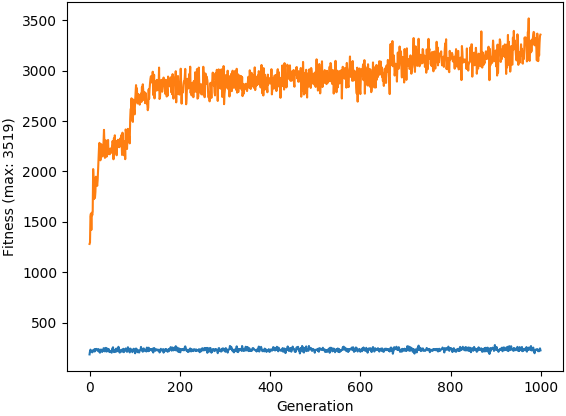
\includegraphics[width=0.5\textwidth]{best-fuzzy-run.png}
    \caption{A plot summarizing the fuzzy run that evolved genomes with the highest training and testing accuracy.  The orange line displays the maximum fitness value per generation.  The blue line displays the average fitness value per generation.}
    \label{bestfuzzyrun}
\end{figure}

\subsection{Denial of Service Attack}

The denial of service evolutionary runs presented challenges that were not discovered with the fuzzy attack runs.  Figure \ref{baddos} displays the results of an evolutionary run with denial of service data and the same binary genome that was used for fuzzy data runs.  The genomes were able to steadily increase fitness values for the first 50 generations.  However, none of the remaining generations made any improvements.  Furthermore, when the resulting evolved genomes were tested against training and testing data, all accuracies were 50\%.  

At first, it was believed that there was a bug in the code.  However, the same code was able to generate acceptable results for runs with fuzzy data.  After further consideration, it occurred that the problem was not based on a bug in the code, but the decision to use a completely binary genome.  As was discussed earlier, denial of service attacks on CAN networks work by injecting messages with an arbitration value of all zeros, which ensures that the injected messages have priority over all other messages.  Therefore, a theoretically optimal binary genome would only care about the bits corresponding to the arbitration value (first 11 bits), and it would be looking for arbitration values of all zero.  However, with this genome, a genuine CAN message with an arbitration value of 64 would look extremely similar to an injected message, as 64 written in binary is 00001000000.  The theoretically optimal binary genome would match with 10 out of the 11 bits in the arbitration value, making the normal message look very similar to the injected messages.  Any genuine CAN message with an arbitration value of a power of two would be treated the same way.  Arbitration values that can be represented by 2 powers of 2, 65 for example (00001000001), would also match very closely with this genome.  Consequently, evolutionary runs with a binary genome will not generate fitness values that push the overall population towards this theoretically optimal binary genome.  Even if it did, the theoretically optimal binary genome would not classify CAN messages with a high accuracy.

It should be noted that the fitness values on the figures in this section do not compare well between figures.  This is because the fitness values depend on how many CAN messages are being used for evaluation (see section III-D for fitness function details).  For example, if the same evolutionary run was performed twice, with the second run using twice the number of messages to generate fitness values, the second run would have fitness values roughly twice as large as the first run.  All three figures in this section used a different number of CAN messages to generate fitness values, so the fitness values alone should not be compared between figures.  

\begin{figure}[h]
    \centering
    \text{Denial of Service Run with Binary-Based Genome}
    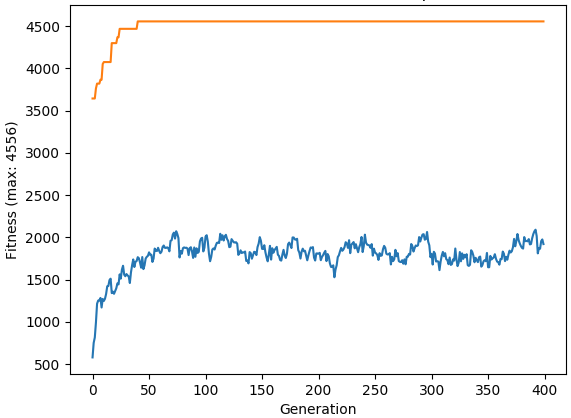
\includegraphics[width=0.5\textwidth]{bad-dos-cropped.png}
    \caption{A plot summarizing a denial of service run using the binary-based genome.  The orange line displays the maximum fitness value per generation.  The blue line displays the average fitness value per generation.}
    \label{baddos}
\end{figure}

After this conclusion was drawn about binary genomes, an integer-based genome was used for the denial of service runs (see section III-B for genome details).  Figure \ref{gooddos} displays a run using the integer-based genome.  At first glance, it appears that the population improves during the first portion of the run and does not make significant improvement for the remainder of the run, as was seen in figure \ref{baddos}.  However, the jump in maximum fitness represents an individual discovering a near optimal solution.  The maximum testing and training accuracies for the evolved genomes from this run were 99.8\% and 99.9\%, respectively.  

\begin{figure}[b]
    \centering
    \text{Denial of Service Run with Integer-Based Genome}
    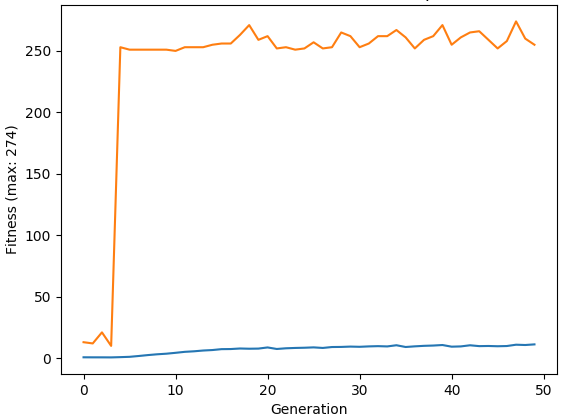
\includegraphics[width=0.5\textwidth]{good-dos-cropped.png}
    \caption{A plot summarizing the denial of service run using an integer-based genome.  The orange line displays the maximum fitness value per generation.  The blue line displays the average fitness value per generation.}
    \label{gooddos}
\end{figure}

\section{Conclusions and Future Work}

The goal of this work was to determine if effective rules for a CAN-based IDS can be evolved.  Considering the results from the previous section, our implementation did not generate high enough overall accuracies to justify its exclusive use to govern an IDS.  While integer-based genomes were able to identify denial of service attacks with a high accuracy, the solution for identifying denial of service attacks on CAN networks was already known.  

However, it is likely that more work on implementation could lead to better performance.  The following items are ideas for future directions:
\begin{itemize}
    \item Evolutionary runs could be performed on data sets with different, or multiple, attack types.  This work only focused on two attack types, and it is possible that evolution could find effective IDS rules for other attack types.
    \item Instead of using binary values in the genome to determine if a section of CAN data is important, evolve decimal values between 0 and 1.  
    \item Make a more flexible genome.  Instead of having genome entries for all sections of CAN data with genome values indicating their importance, have a genome of variable length where entries indicate what section of data to look at and what value to check for at that location.  
    \item Implement a way to process time stamp values in the genome.
\end{itemize}

\bibliographystyle{ieeetr}
\bibliography{refs}

\end{document}
